\chapter{Event selection and analysis strategy} %day1
\label{chap:selection}

Given the theoretical motivation for \BSM physics in
Chapter~\ref{chap:theory}, the next Chapters of this thesis describe a
search for \SUSY with the \CMS detector in $13~\tev$ proton collisions
produced by the \LHC. The analysis is designed to target \SUSY
produced in a strong force interaction that decays hadronically via
\SM particles to a weakly interacting \LSP. The typical \SUSY models
considered in this search are those with gluino or squark pair
production. However, it is possible to generalise the search to look
for any \BSM signatures that have a weakly interacting particle with
significant momentum in the final state.
% introduce analysis and what the next chapters are about
% hadronic, inclusive, targets gluino and squark production but can be
% generalised to DM

As \SUSY has a significant number of free parameters, it can manifest
itself in a wide range of decay topologies. For this reason the
analysis is aimed to be as inclusive as possible, covering as much
parameter space as is feasible.  This is dictated by an ability to
predict the backgrounds from \SM processes with minimal uncertainties.
The search then attempts to find statistically significant excesses in
the data counts above those predicted for the various backgrounds. To
maximise the chance of seeing \BSM phenomena events are typically
required to have significant hadronic activity and missing momentum.  
% Robust strategy - minimise background uncertainties and look for
% excesses on top, in a conservative way (be very general here)


%%%%%%%%%%%%%%%%%%%%
\section{Challenges for a hadronic \BSM search}
\label{sec:challenge}

%main challenge in limiting and understanding backgrounds
The main challenge for a hadronic \BSM search is in limiting and
understanding the backgrounds, while maximising acceptance of a wide
range of potential \BSM signals. Within the analysis presented in this
Chapter the backgrounds are considered in two separate categories,
either as coming from a QCD multijet process or from a \SM process
with genuine \MET. As the search can look for generic signs of
excesses that are indicative of \BSM processes, considerations of the
modelling of the signal models are not as important as constraining
and understanding these backgrounds.

\subsection{The QCD multijet background}
\label{sec:qcdMultijet}

The most abundant \SM process in $pp$-collisions at the \LHC is \QCD
multijet production through strong force interactions. This background
is orders of magnitude greater than other processes, as is evident
from the total \LHC cross section in Fig.~\ref{fig:xsecs}. The
majority of the \QCD background consists of events with multiple jets,
most commonly two, produced in a balanced configuration, with no
significant missing momentum, \MET or \MHT. A requirement on these
variables therefore significantly reduces the background. As
the abundance of such events is so large, however, mismeasurement of
the jets can lead to a significant \QCD background passing such
requirements. The fake missing energy can be introduced in a variety
of ways:
\begin{itemize}
\item{Effects in the detector leading to inefficiencies, such as jets
falling into regions of the detector that or uninstrumented or have a
reduced response due to hardware issues.}
\item{Fake additional energy being introduced. This can occur through
detector malfunctions, for example from problems in the readout
electronics. It can also be introduced through \PU that is attributed to
the primary vertex. Additionally beam interactions that produce
particles outside the detector can lead to mismeasurement.}
\item{Issues at the reconstruction stage can also introduce fake \MET,
such as through under or over-corrections of jet energies, or through
the reconstruction algorithms missing physics objects that are
produced.}
\item{Physics objects with energies that fall below their selection
threshold can also artificially introduce missing energy signatures,
particularly when there is a collection of them pointing in a similar
direction.}
\end{itemize}

The ways in which this fake missing energy can be introduced are
taken account of in as many ways as possible. However, due to the
nature of these effects, which is often time dependent, they cannot be
fully accounted for in simulation. This fact, coupled with the
difficulty in accurately simulating \QCD processes due to theoretical
uncertainties, makes constraining the multijet background a significant
challenge. 

It is also possible for the \QCD multijet background to be produced in
association with genuine \MET. This occurs in the case of \emph{heavy
flavour} \QCD, where a $b\bar{b}$ quark pair are produced and at least
one the $b$-quarks decay via the weak force, producing a neutrino.
This is subdominant to the mismeasured multijet background, but must
still be accounted for. 
% heavy flavour qcd

% relevant to the trigger (cite back advantages from trigger chapter)

\subsection{Backgrounds from standard model processes with genuine
\MET}

The other class of \SM backgrounds are those produced with genuine
\MET. These processes only occur in the \SM through the electroweak
production of neutrinos and can be denoted as \emph{EWK}. Due to the
mass scale of such electroweak processes, they commonly occur in
association with jets of a significant momentum. The dominant
processes that constitute this background are \wj, \znunu and \ttbar,
with residual backgrounds from other, lower cross section,
vector-boson or top production processes.

As a hadronic analysis does not look for leptons in the final state,
vetoing isolated leptons can help to reduce the background from the
\wj and \ttbar processes. In these cases a lepton is always produced
in association with the neutrino that results in the significant \MET.
Such events will only present a problem when the leptons are not
reconstructed, or do not appear to be isolated.  If the $W$ boson
decays via a \tau-lepton that subsequently decays hadronically the
event will not be removed by the lepton veto.  This is a comparably
small background, however.

The major irreducible background in \BSM searches with \MET comes from 
\znunu processes. They produce a pure missing energy signature with no
associated leptons to veto. Understanding this background to a high
degree of accuracy constitutes a significant challenge. Due to the
better simulation of electroweak processes compared to \QCD processes,
this background can be understood with smaller uncertainties than the
\QCD background.
% Z nu nu
%plots with backgrounds: http://www.hep.ph.ic.ac.uk/~mc3909/procs/

%%%%%%%%%%%%%%%%%%%%
\section{The \alphat analysis} 

The search for \SUSY described within this thesis revolves around
suppression of the \QCD multijet background to negligible levels
through the use of topological variables, including \alphat,
described in Sec.~\ref{sec:topoVars}. With negligible \QCD the
large uncertainties that are usually prevalent when predicting this
background are greatly reduce. The use of these topological variables
also provides robustness against a wide range of mismeasurement
effects, which are particularly relevant when looking at early data
when the detector is not as well understood. The remaining background
from electroweak processes is then estimated in a \emph{data-driven} way,
minimising the uncertainties from relying on simulation.

During Run~1 of the \LHC the \alphat analysis has been performed
extensively to search for \SUSY. Datasets of $4.98~\ifb$ at
$\sqrt{s}=7~\tev$ and $18.5~\ifb$ at $\sqrt{s}=7~\tev$ have been
analysed, setting limits on \SUSY production within the context of
simplified models
\cite{Chatrchyan:2011zy,Khachatryan:2011tk,Chatrchyan:2012wa,Chatrchyan:2013mys,Khachatryan:2016pxa}.
The analysis presented within this thesis is performed on the data
collected during Run~2 of the \LHC at $\sqrt{s}=13~\tev$. The analysis
has been redesigned and optimised to perform well at the higher centre
of mass energy. Significant improvements have been made to improve the
sensitivity of the analysis and in characterising the various
backgrounds.

%%%%%%%%%%%%%%%%%%%%
\section{QCD multijet suppression with topological variables} %day2
\label{sec:topoVars}

As discussed in Sec.~\ref{sec:qcdMultijet}, a pure requirement on the
\MET of an event is not always enough to remove the \QCD multijet
background.  To effectively remove it, the mismeasurement that leads
to the fake \MET signature must be identified and used to remove
mismeasured events. This can be achieved by making use of topological
variables, which use specific facts about the topology of an event to
decide whether the \MET comes from mismeasurement or a weakly
interacting particle. 
%why topological variables work!! - fake met from detector cock ups

\subsection{The \alphat variable}
%introduce the variables and why they're useful

The dimensionless variable, \alphat, was originally proposed as the
$\alpha$ variable \cite{Randall:2008rw}, but changed to a transverse
quantity to make it more suitable for use in a hadron collider
\cite{CMS-PAS-SUS-08-005,CMS-PAS-SUS-09-001}. It is intrinsically
robust against jet energy mismeasurements in multijet systems. For a
dijet system, \alphat is defined as: 
\begin{equation}
\alpha_T=\frac{E_T^{j_2}}{M_T}, 
\end{equation} 
where $E_T^{j_2}$ is the transverse energy of the lower energy jet and
$M_T$ is the invariant mass of the dijet
system, defined as:
\begin{equation}
M_T=\sqrt{(\Sigma E_T^{j_i})^2-(\Sigma p_x^{j_i})^2-(\Sigma
p_y^{j_i})^2},
\end{equation}
where $E_T^{j_i}$ is the transverse energy of jet, $j_i$ and the $x$
and $y$ components of the transverse momentum are $p_x^{j_i}$ and
$p_y^{j_i}$ respectively.

In the case that the event in question is a perfectly measured dijet
event $E_T^{j_1}=E_T^{j_2}$ and both jets are back-to-back in $\phi$.
This results in a value of $\alphat=0.5$ when the momentum of each jet
is large in comparison with its mass, as is usually the case in
\QCD multijet events. If the jets are still back-to-back but one of
them is mismeasured, this will result in a value of $\alphat<0.5$.
However, in the case that the two jets are recoiling from a genuine
source of \MET, they will not be back-to-back and generally $\alphat>0.5$.

For events with more than two jets, a \emph{pseudo dijet} system is
formed by summing jets vectorially to combine them.  The system chosen
is one that minimises $|\Delta E_T|$, the difference between the $E_T$
of each pseudo jet, where $E_T$ is the scalar sum of the transverse
energies of all the jets in each pseudo jet. This form of clustering
is chosen as it forms the most balanced configuration, making the
pseudo dijet event appear as close to an event with no mismeasurement
as possible. It leads to a generalised form of $\alpha_T$: 
\begin{equation}
\alpha_T=\frac{\Sigma E_T^{j_i}-\Delta
E_T}{2\sqrt{(\Sigma E_T^{j_i})^2-\cancel{H}_T^2}}.
\end{equation} 
In the case that there is no mismeasurement or \MET, $\Delta
E_T=\MET=0$ and $\alphat=0.5$. However, if the energy of the jets is
mismeasured, the value of $\Delta E_T$ will be very close to \MET,
resulting in $\alphat<0.5$. When the jets are recoiling from genuine
\MET, $\Delta E_T\sim 0$ and $\alphat>0.5$.
  
The efficacy of an $\alphat$ cut in removing the \QCD multijet
background is evident in Fig.~\ref{fig:alphaT}. By
choosing an appropriate cut above $0.5$ it is possible to reduce the
multijet background to a negligible level.

% put more upt to date one here
\begin{figure}
	\begin{center}
		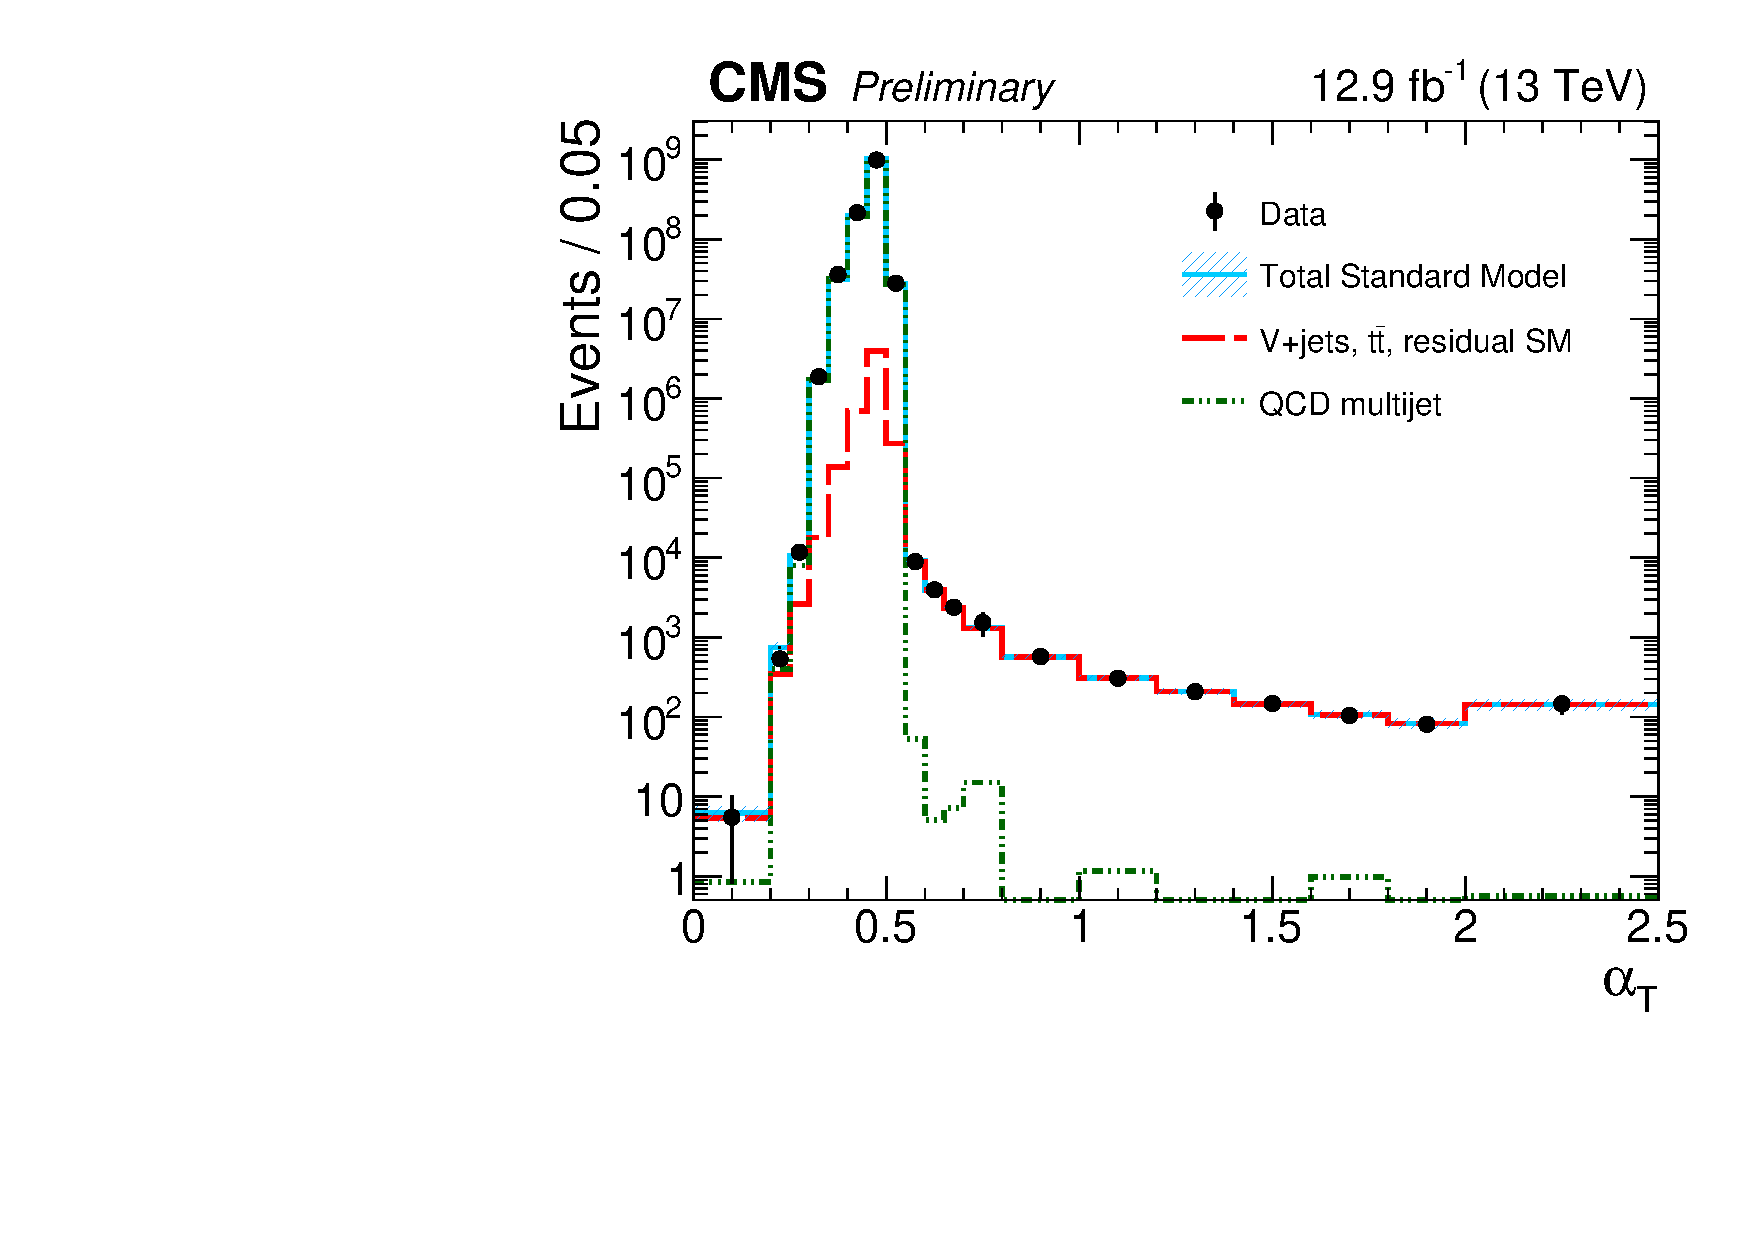
\includegraphics[width=0.8\linewidth]{figs/analysis/eventSelection/CMS-PAS-SUS-16-016_Figure-aux_001}%alphaT1_bkgd}
	\end{center}
  \caption{The $\alpha_T$ distribution for events with $H_T>200$ GeV
  that pass the pre-selection criteria (Sec.~\ref{sec:preselection}) when
  $\alphat<0.55$ and the signal selection criteria
  (Sec.~\ref{sec:signalregion}) when
  $\alphat>0.55$. The green dotted line shows the expected multijet
  QCD background that can be removed with an appropriate cut on
  $\alpha_T$}
	\label{fig:alphaT}
\end{figure}

\subsection{The \bdphi variable}

% introduce and explain

% show the plot from Mark

%put the stuff about bDPhi over dPhi as in the ICHEP note

\subsection{$\MHT/\MET$}

% removes soft stuff! given jet threshold


%%%%%%%%%%%%%%%%%%%%
\section{Physics objects} %day3

%surely comes from the note?

% tracks + vertices
%SITV

% jets
% how we construct HT,MHT,MET

% muons

% electrons

%%%%%%%%%%%%%%%%%%%%
\section{Trigger strategy}

%big shit loads of QCD

%L1

%HLT

% justify corrections etc.

%%%%%%%%%%%%%%%%%%%%
\section{Event selection and categorisation} %day4

\subsection{Pre-selection}
\label{sec:preselection}

%work in progress from 18 month:
The only genuine source of missing transverse energy ($\cancel{E}_T$)
in the SM is electroweak neutrino production. In these cases, with the
exception of a $Z$ decaying via a pair of neutrinos, an associated
lepton is simultaneously produced. This background is minimised by
vetoing any events with isolated \footnote{A particle is isolated if
the energy of other particles within a cone of
$R\equiv\sqrt{(\Delta\phi)^2+(\Delta\eta)^2}=0.3$, where $\phi$ is the
azimuthal angle and $\eta$ the pseudorapidity, do not add up to a
significant proportion of the particle's momentum, typically
$\sim10$\%} leptons of $p_T>10$~GeV. To ensure a fully hadronic final
state there is also a veto on photons of $p_T>25$~GeV. Further, to
reduce the ``lost lepton'' backgrounds from W~+~jets and $t\bar{t}$,
events containing single isolated tracks with $p_T >10$~GeV and
$|\eta| < 2.5$ are vetoed.

Events are also required to contain at least one $p_T>100$~GeV and one
$p_T>40$~GeV jet, where the jets are well reconstructed in the central
region, $|\eta|<3$. If any jets fall outside the $\eta$ range, the
event is vetoed. Significant hadronic activity is selected by
requiring $H_T>200$~GeV. Events are categorised based on the number of
jets, the number of jets with a reconstructed b-quark and the value of
$H_T$. 

\subsection{The signal region}
\label{sec:signalregion}

%variable alphaT
%bDphi

\subsection{The control regions}

%describe and motivate each of them as in AN

\subsection{Event categorisation}

%the jet topology, symmetric, asymmetric etc.

%%%%%%%%%%%%%%%%%%%%
\section{Corrections to simulation} %day5

% mention tails of Njet and ETmiss are hard to simulate?


\subsection{Trigger efficiencies}

% put in trigger efficiency plots

\subsection{Scale factors}

% SFs from muons etc...

%%%%%%%%%%%%%%%%%%%%
%\section{Further optimisation of event selection}
% something about minChi here?
